\section{Descripción teórica}

\subsection{Linea de transmisión bifilar}
Una línea de transmisión bifilar es un tipo de conductor eléctrico compuesto por dos hilos paralelos separados por un dieléctrico. Este tipo de línea es ampliamente utilizado en diversas aplicaciones de telecomunicaciones debido a su simplicidad constructiva y sus características de transmisión.

\subsection{Impedancia Característica}

Uno de los parámetros más importantes de una línea de transmisión es la impedancia característica ($Z_o$). Esta representa la relación entre el voltaje y la corriente que se propaga a lo largo de la línea en modo transversal electromagnético (TEM). La impedancia característica de una línea bifilar depende de la geometría de los conductores (diámetros y separación) y de las propiedades del dieléctrico (permitividad relativa).
        \begin{center}
        \begin{figure}[H]
        \centering  
        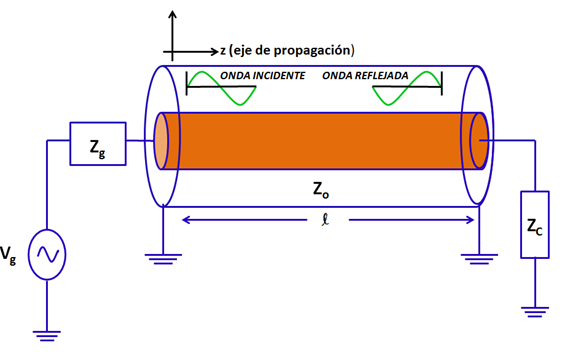
\includegraphics[scale=0.7]{imagenes/Modelo esquemático de una línea de transmisión conectada.png}
        \caption{Modelo esquemático de una línea de transmisión conectada}
        \end{figure}
        \end{center}

\subsection{Velocidad de Propagación}

La velocidad de propagación de una onda electromagnética a lo largo de una línea de transmisión es menor que la velocidad de la luz en el vacío y depende de la permitividad relativa del dieléctrico. Esta velocidad se relaciona con la longitud de onda de la señal y el período de la misma.
        \begin{center}
        \begin{figure}[H]
        \centering  
        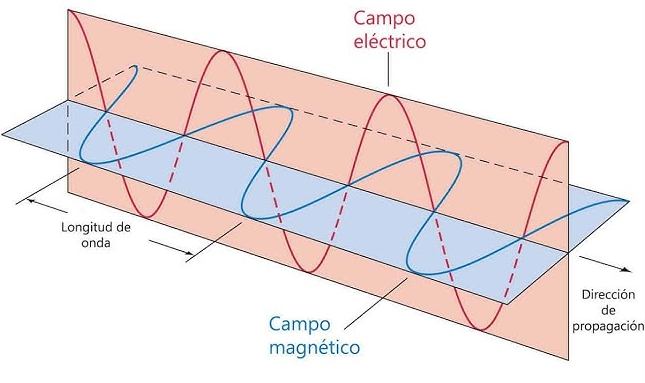
\includegraphics[scale=0.7]{imagenes/propagacion de una onda electromagnetica.png}
        \caption{Propagación de una onda electromagnética}
        \end{figure}
        \end{center}
\subsection{Atenuación}

La atenuación representa la pérdida de potencia de la señal a medida que se propaga a lo largo de la línea. Esta pérdida se debe a varios factores, como la resistencia óhmica de los conductores, las pérdidas dieléctricas y las pérdidas por radiación. La atenuación se expresa en decibelios por unidad de longitud (dB/m).

\subsection{Capacitancia y Inductancia en una linea de transmisión bifilar}

Una línea de transmisión bifilar puede ser modelada como una sucesión infinita de elementos infinitesimales, cada uno compuesto por una inductancia y una capacitancia. La capacitancia se debe a la presencia del campo eléctrico entre los conductores, mientras que la inductancia se debe al campo magnético generado por la corriente que circula por los conductores.

\subsection{Modelo de Línea de Transmisión}

Para analizar el comportamiento de una línea de transmisión, se utiliza el modelo de línea de transmisión distribuida, que considera la distribución continua de los parámetros a lo largo de la línea. Este modelo permite obtener las ecuaciones de telegrafistas, que relacionan el voltaje y la corriente en cualquier punto de la línea.

        \begin{center}
        \begin{figure}[H]
        \centering  
        \includegraphics[scale=1]{imagenes/Modelo de parámetros distribuidos.png}
        \caption{Modelo de parámetros distribuidos}
        \end{figure}
        \end{center}

        \begin{center}
        \begin{figure}[H]
        \centering  
        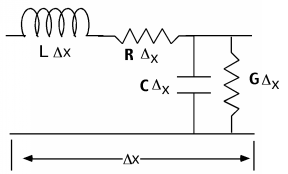
\includegraphics[scale=1]{imagenes/Modelo distribuido completo.png}
        \caption{Modelo distribuido completo}
        \end{figure}
        \end{center}
%\subsetion{Línea bifilar (altas frecuencias)}[\cite{hayt}] %se le agrega [1] según la bibliografia o \cite{nombre}

\begin{comment}Para la línea de transmisión bifilar que muestra la figura \ref{fig:linea-bifilar} con conductores de radio a y
conductividad σc con una separación entre centros igual a d y un medio de permeabilidad μ,

que la capacitancia está dada por \end{comment}

\begin{comment}
\subsection{Relación con el Problema}
permitividad , y conductividad σc, se encontró en el capítulo 6 [ecuación (40), sección 6.5]
En este trabajo, los conceptos teóricos mencionados anteriormente se aplicarán para diseñar una línea de transmisión bifilar que cumpla con las especificaciones establecidas. Se utilizarán las ecuaciones de línea de transmisión para calcular las dimensiones geométricas de la línea y verificar que se obtenga la impedancia característica, la capacitancia y la velocidad de propagación deseadas. Además, se analizarán las pérdidas en la línea para evaluar el cumplimiento de la especificación de atenuación.

Esta sección puede ser ampliada o modificada según tus necesidades. Puedes agregar más detalles sobre los conceptos que consideres relevantes, como:

\textbf{Modos de propagación:} Explicar brevemente los diferentes modos de propagación en líneas de transmisión y por qué se considera el modo TEM en este caso.
\textbf{Coeficiente de reflexión:} Definir el coeficiente de reflexión y su importancia en el diseño de líneas de transmisión.
\textbf{Adaptación de impedancias:} Explicar la importancia de adaptar la impedancia de la línea a la impedancia de la carga para evitar reflexiones.
\end{comment}

\pagebreak
